\documentclass[10pt, a4paper]{article}
% \usepackage[english]{babel}
\usepackage[brazilian]{babel}
\usepackage[utf8]{inputenc}
% \usepackage[T1]{fontenc}

% matlab code
% \usepackage{matlab-prettifier}
\usepackage[numbered,framed]{matlab-prettifier}
\renewcommand{\lstlistingname}{C\'odigo} % Listing->Code
\let\ph\mlplaceholder % shorter macro
\definecolor{codegreen}{rgb}{0,0.6,0}
\definecolor{codegray}{rgb}{0.5,0.5,0.5}
\definecolor{codepurple}{rgb}{0.58,0,0.82}
\definecolor{backcolour}{rgb}{0.95,0.95,0.92}
\lstdefinestyle{myStyle}{
%     belowcaptionskip=1\baselineskip,
    language=Matlab,
    breaklines=true,
    frame=single,
    numbers=none,
    basicstyle=\tiny\ttfamily,%\footnotesize\ttfamily,
    keywordstyle=\bfseries\color{magenta},
    commentstyle=\color{codegreen},
    identifierstyle=\color{blue},
    backgroundcolor=\color{backcolour},
    stringstyle=\color{codepurple},
}
\usepackage{adjustbox}

% For subfigure use
\usepackage[font=small,labelfont=bf]{caption}
\usepackage{subcaption}

% Set page size and margins
% Replace `letterpaper' with`a4paper' for UK/EU standard size
\usepackage[a4paper,top=2cm,bottom=2cm,left=2cm,right=2cm,marginparwidth=2cm]{geometry}

% tabelas
\usepackage{array}
\usepackage{tabularx}
\usepackage{booktabs}

\usepackage{float}

% Useful packages
\usepackage{amsmath}
\usepackage{undertilde}
\usepackage{graphicx}
\graphicspath{{figures/}} %Setting the graphicspath
\usepackage[colorlinks=true, allcolors=blue]{hyperref}

\title{PUC-RJ Pontif\'icia Universidade Cat\'olica do Rio de Janeiro \\ MEC 2403 - Otimiza\c c\~ao e Algoritmos para Engenhria Mec\^anica \\ Trabalho 01 - Otimiza\c c\~ao  sem Restri\c c\~oes  \\
\large Professor: Ivan Menezes}

\author{Felipe da Costa Pereira - mat. 2212376 \\ {\tt felipecostapereira@gmail.com}}
\begin{document}

\maketitle

\section{Introdu\c c\~ao}

Otimiza\c c\~ao sem restri\c c\~ao (OSR) consiste em encontrar o m\'inimo de uma fun\c c\~ao $f(\vec{x})$ onde n\~ao h\'a restri\c c\~ao em rela\c c\~ao ao dom\'inio das vari\'aveis $\vec{x}$. A fim de se encontar o minimo da fun\c c\~ao $f(\vec{x})$ a partir de um ponto de partida $(\vec{x_{0}})$ , os m\'etodos apresentados nesse trabalho consistem na repeti\c c\~ao de duas etapas principais at\'e que um crit\'erio de parada seja atingido:
\begin{enumerate}
      \item Selecionar uma dire\c c\~ao $\vec{d}$ a partir do ponto $\vec{x_{0}}$
      \item Encontrar o m\'inimo da fun\c c\~ao $f$ nessa dire\c c\~ao, chegando a um novo ponto $\vec{x_{1}} = \vec{x_{0}} + \alpha\vec{d}$, onde $\alpha$ \'e um n\'umero real.
      \item Tomar $\vec{x_{1}}$ como o novo ponto de partida $\vec{x_{0}}$
      \item Repetir os passos de 1 a 3 at\'e que uma condi\c c\~ao de parada seja atingida: m\'inimo encontrado ($|\vec{\nabla f}|=0$), ou m\'aximo n\'umero de itera\c c\~oes atingido.
\end{enumerate}

Dessa forma o problema de minimiza\c c\~ao da fun\c c\~ao $f(\vec{x})$ se torna um problema de sucessivas determina\c c\~oes de dire\c c\~oes de busca e suas respectivas buscas lineares nesssas dire\c c\~oes.

\section{Objetivos}

Os principais objetivos deste trabalho s\~ao:
\begin{itemize}
      \item Implementar numericamente os algoritmos de otimiza\c c\~ao: Univariante, Powell, Steepest Descent, Fletcher-Reeves, Newton-Raphson e BFGS.
      \item Avaliar a influ\^encia dos par\^ametros dos algoritmos nas m\'etricas de converg\^encia e comparar essas \'ulltimas com os valores esperados da teoria.
      \item Aplicar os algoritmos implementados na solu\c c\~ao do problema de OSR em tr\^es casos: uma fun\c c\~ao quadr\'atica, uma n\~ao quadr\'atica e uma terceira fun\c c\~ao que representa um problema de engenharia (minimizaz\c c\~ao da energia de um sistema massa-mola visando encontrar seu ponto de equil\'ibrio est\'atico)
\end{itemize}

\section{Algoritmos de Busca Linear}

Os algoritmos de minimiza\c c\~ao s\~ao executaodos em duas etapas conforme citado anteriormente: uma primeira etapa consiste em determinar dire\c c\~oes de busca $\vec{d}$ e minimizar a fun\c c\~ao $f$ nessa dire\c c\~ao, de forma unidimensional, o que significa encontrar o valor de  $\alpha$ que minimiza a fun\c c\~ao $f(x=x_{0}+\alpha\vec{d})$ ao longo da dire\c c\~ao $\vec{d}$. A busca linear \'e relizada em duas etapas: Passo constante e refinamento do c\'alculo de $\alpha$.

\subsection{Passo Constante}

A primeira etapa da busca linear consiste numa busca inexata que visa encontrar um intervalo de valores do passo $\alpha$, $[\alpha_{L}, \alpha_{H}]$ que represente uma redu\c c\~ao suficientemente grande da fun\c c\~ao $f$. Essa implementa\c c\~ao num\'erica incrementa o passo de um valor $d\alpha$ at\'e que a fun\c c\~ao pare de diminuir.

\subsection{Bisse\c c\~ao e Se\c c\~ao \'Aurea}

Ap\'os a etapa do passo constante, os m\'etodos da Bisse\c c\~ao ou Se\c c\~ao \'Aurea s\~ao aplicados para encontrar o valor de $\alpha$, entre os valores determinados no intervalo da etapa 1. Em ambos os casos, o intervalo de ocorr\^encia do valor m\'inimo de $f$ \'e sucessivamente reduzido at\'e que seja muito pequeno e considera-se, dado esse crit\'erio num\'erico, solucionado o problema da minimiza\c c\~ao de $f$ nessa dire\c c\~ao, encontrando o passo $\alpha_{k}$ correspondente a esse m\'inimo.

O m\'etodo da bisse\c c\~ao divide sucessivamente o intervalo descartando a parte superior ou inferior do mesmo avaliando o valor da fun\c c\~ao $f$ na vizinhan\c ca esquerda e direita de um $\alpha_{M}$ m\'edio do intervalo. J\'a o m\'etodo da se\c c\~ao \'aurea utiliza a raz\~ao \'aurea para descarte dos intervalos onde $f$ aumenta. Este \'ultimo m\'etodo realiza mais passos, por\'em possui a vantagem de avaliar menos vezes a fun\c c\~ao $f$ uma vez que os valores avaliados no passo anterior podem ser reutilizados no passo seguinte do algoritmo, o que pode ser interessante em problemas onde a avalia\c c\~ao da fun\c c\~ao $f$ \'e computacionalmente cara.

\section{Algoritmos de Dire\c c\~ao}

Conforme descrito anteriormtente, os m\'etodos de dire\c c\~ao determinam dire\c c\~oes de busca do m\'inimo de $f$ a partir de um ponto $\vec{x_{k}}$. A partir da busca linear encontra-se o valor do passo nessa dire\c c\~ao que minimiza $f$, ($\alpha_{k}$), os algoritmos de dire\c c\~ao calculam, ent\~ao, a pr\'oxima dire\c c\~ao onde se deve minimizar $f$ e a partir do novo ponto $\vec{x_{k+1}}=\vec{x_k}+\alpha_{k}\vec{d}$. O processo se repete at\'e que uma condi\c c\~ao de parada seja atingida.

\subsection{Univariante}

O m\'etodo univariante \'e o mais simples, onde as dire\c c\~oes de busca s\~ao as dire\c c\~oes can\^onicas, $\vec{d_{k}}=\vec{e_{k}}$.

\subsection{Powell}

O m\'etodo de Powell utiliza em seu algoritmo dire\c c\~oes denominadas "movimento padr\~ao". O m\'etodo de Powell gera dire\c c\~es Q-conjugadas, o que representa uma acelera\c c\~ao em rela\c c\~ao ao m\'etodo univariante. O m\'etodo de Powell converge para o m\'inimo de uma fun\c c\~ao quadr\'atica $n$ vari\'aveis em um n\'umero finito de passos dado por $n+1$ (notas de aula).

\subsection{Steepest Descent}

O m\'etdo Steepest Descent \'e um m\'etodo onde as dire\c c\~oes s\~ao dadas pela dire\c c\~ao oposta ao gradiente da fun\c c\~ao $f$. Ou seja, $\vec{d_{k}} = -\vec{\nabla} f(\vec{x_{k}})$.

\subsection{Fletcher-Reeves}

Este m\'etodo consiste em uma adapta\c c\~ao do m\'etodo dos Gradientes Conjugados que o torna capaz de ser usado para minimiza\c c\~ao de uma fun\c c\~ao qualquer. Para anto, duas modifica\c c\~oes precisam ser realizadas, a avaliacao da matriz Q (ou Hessiana para funcao nao quadratica) \'e substituida por uma busca linear e o parametro $\beta$ modificado (notas de aula)

\subsection{Newton-Raphson}


\subsection{BFGS}

\section{Metodologia}

Para atingir os objetivos do trabalho, foram programados scripts em linguagem Matlab, organizados conforme esquematizado na figura \ref{fig:fluxo}.

\begin{figure}[H]
      \centering
      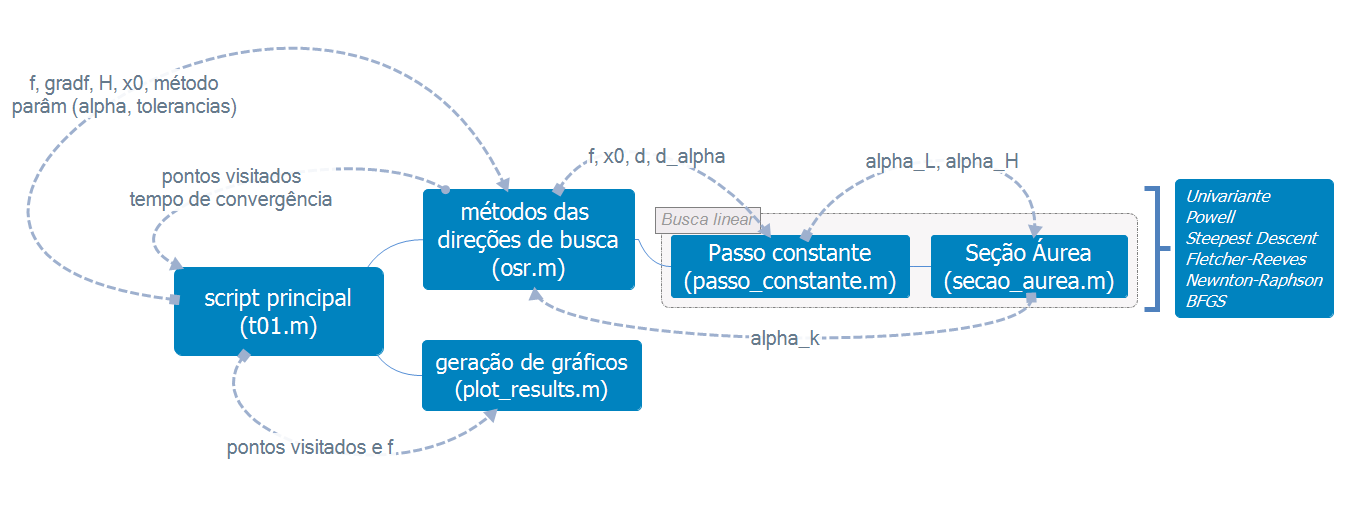
\includegraphics[width=.9\textwidth]{t01.png}
      \caption{Fluxo dos scripts}
      \label{fig:fluxo}
\end{figure}

Um script principal \textit{t01.m} escolhe os par\^ametros do algoritmo: $\alpha$ da busca linear, m\'aximo n\'umero de itera\c c\~oes e toler\^ancias para avaliar a converg\^encia. Al\'em disso esse script cria as fun\c c\~oes, seus gradientes, matriz Hessiana e pontos iniciais, a serem passados como par\^ametros para o script que implementa os algoritmos, conforme ilustrado na listagem \ref{l1} da se\c c\~ao Anexos.

Em seguida, o script \textit{t01.m} chama o script \textit{osr.m} para cada m\'etodo e plota as curvas de n\'ivel da fun\c c\~ao f e todos os pontos visitados durante a busca do algoritmo, atrav\'es do script \textit{plot\_result.m} (listagem \ref{l2})

O script \textit{osr.m} implementa de fato os algoritmos a partir dos par\^ametros recebidos, retornando todos os valores de $\vec{x}$ visitados e o tempo de execu\c c\~ao. A listagem de c\'odigo \ref{list_osr} ilustra a implementa\c c\~ao do algoritmo de Powell.

Outros dois scripts invocados na solu\c c\~ao dos problemas propostos s\~ao \textit{passo\_constante.m} e \textit{secao\_aurea.m}, que realizam a etapa de busca linear para cada dire\c c\~ao de busca. Esses c\'odigos s\~ao listados nas listagens \ref{list_passo_constante} e \ref{list_secao_aurea}, respectivamente.

\section{Resultados}

\section{Conclu\~oes}

In order to use the Tustin model for the friction force as proposed, the torque expression changes from equation \ref{eq:1} to equation \ref{eq:2} described below:     \newline


Torque expression using Coulomb friction force model:
\begin{equation}\label{eq:1}
      \tau(t) = M\ddot{q}(t) + F_{v}\dot{q}(t) + F_{c}sign(\dot{q}(t)) + offset
\end{equation}

Torque expression using Tustin friction force model:
\begin{equation}\label{eq:2}
      \tau(t) = M\ddot{q}(t) + F_{v}\dot{q}(t) + F_{c}sign(\dot{q}(t)) + (F_{s} - F_{c})e^{-\frac{|\dot{q}|}{v_{s}}} + offset
\end{equation}


Parameters and $\dot{x_{2}}=\ddot{q}$ expresion on the state vector: \\

The range for the $v_{s}$ parameter was based on the respecitve value given by the IDIM model ($v_{s} = 0.006464$). The rest of the code is kept exactly the same.

\section{Results}

After performing the grey box identification using the casadi library, we compare the parameters values estimated by the inverse dynamic model (IDM) and the grey box casadi model. The values of the estiamted parameters, for both the Coulomb and the Tustin friction forces are shown in tables \ref{table:m1} and \ref{table:m2}.

\begin{table}[H]
      \small
      \centering
      \caption{Coulomb Model parameters}
      \begin{tabular}{c|c|c|c|c}
            Model &  M & Fv & Fc & ofst \\
            \hline
            casadi & 95.1089 & 203.5034 & 20.3935 & -3.1648 \\
            IDIM   & 96.0014 & 213.8943 & 19.4167 & -3.2790 \\
      \end{tabular}
      \label{table:m1}
\end{table}

\begin{table}[H]
      \small
      \centering
      \caption{Tustin Model parameters}
      \begin{tabular}{c|c|c|c|c|c|c}
            Model &  M & Fv & Fc & Fs & vs & ofst \\
            \hline
            casadi & 97.001 & 222.01 & 18.606 & 36.3311 & 0.000900 & -3.29 \\
            IDIM   & 95.681 & 203.36 & 17.023 & 17.0230 & 0.006464 & -4.12 \\
      \end{tabular}
      \label{table:m2}
\end{table}

The simulated responses and the associeted errors, for both force models (Coulomb and Tustin) and parameters estimation methods (casadi amd IDIM) are show in figures \ref{fig:y} and \ref{fig:e}.

As we can notice, casadi models estimate have a good fit for both force models, while IDIM models have a poor performace (higher error) when estimating the Tustin force model parameters.

\begin{figure}[H]
      \centering
      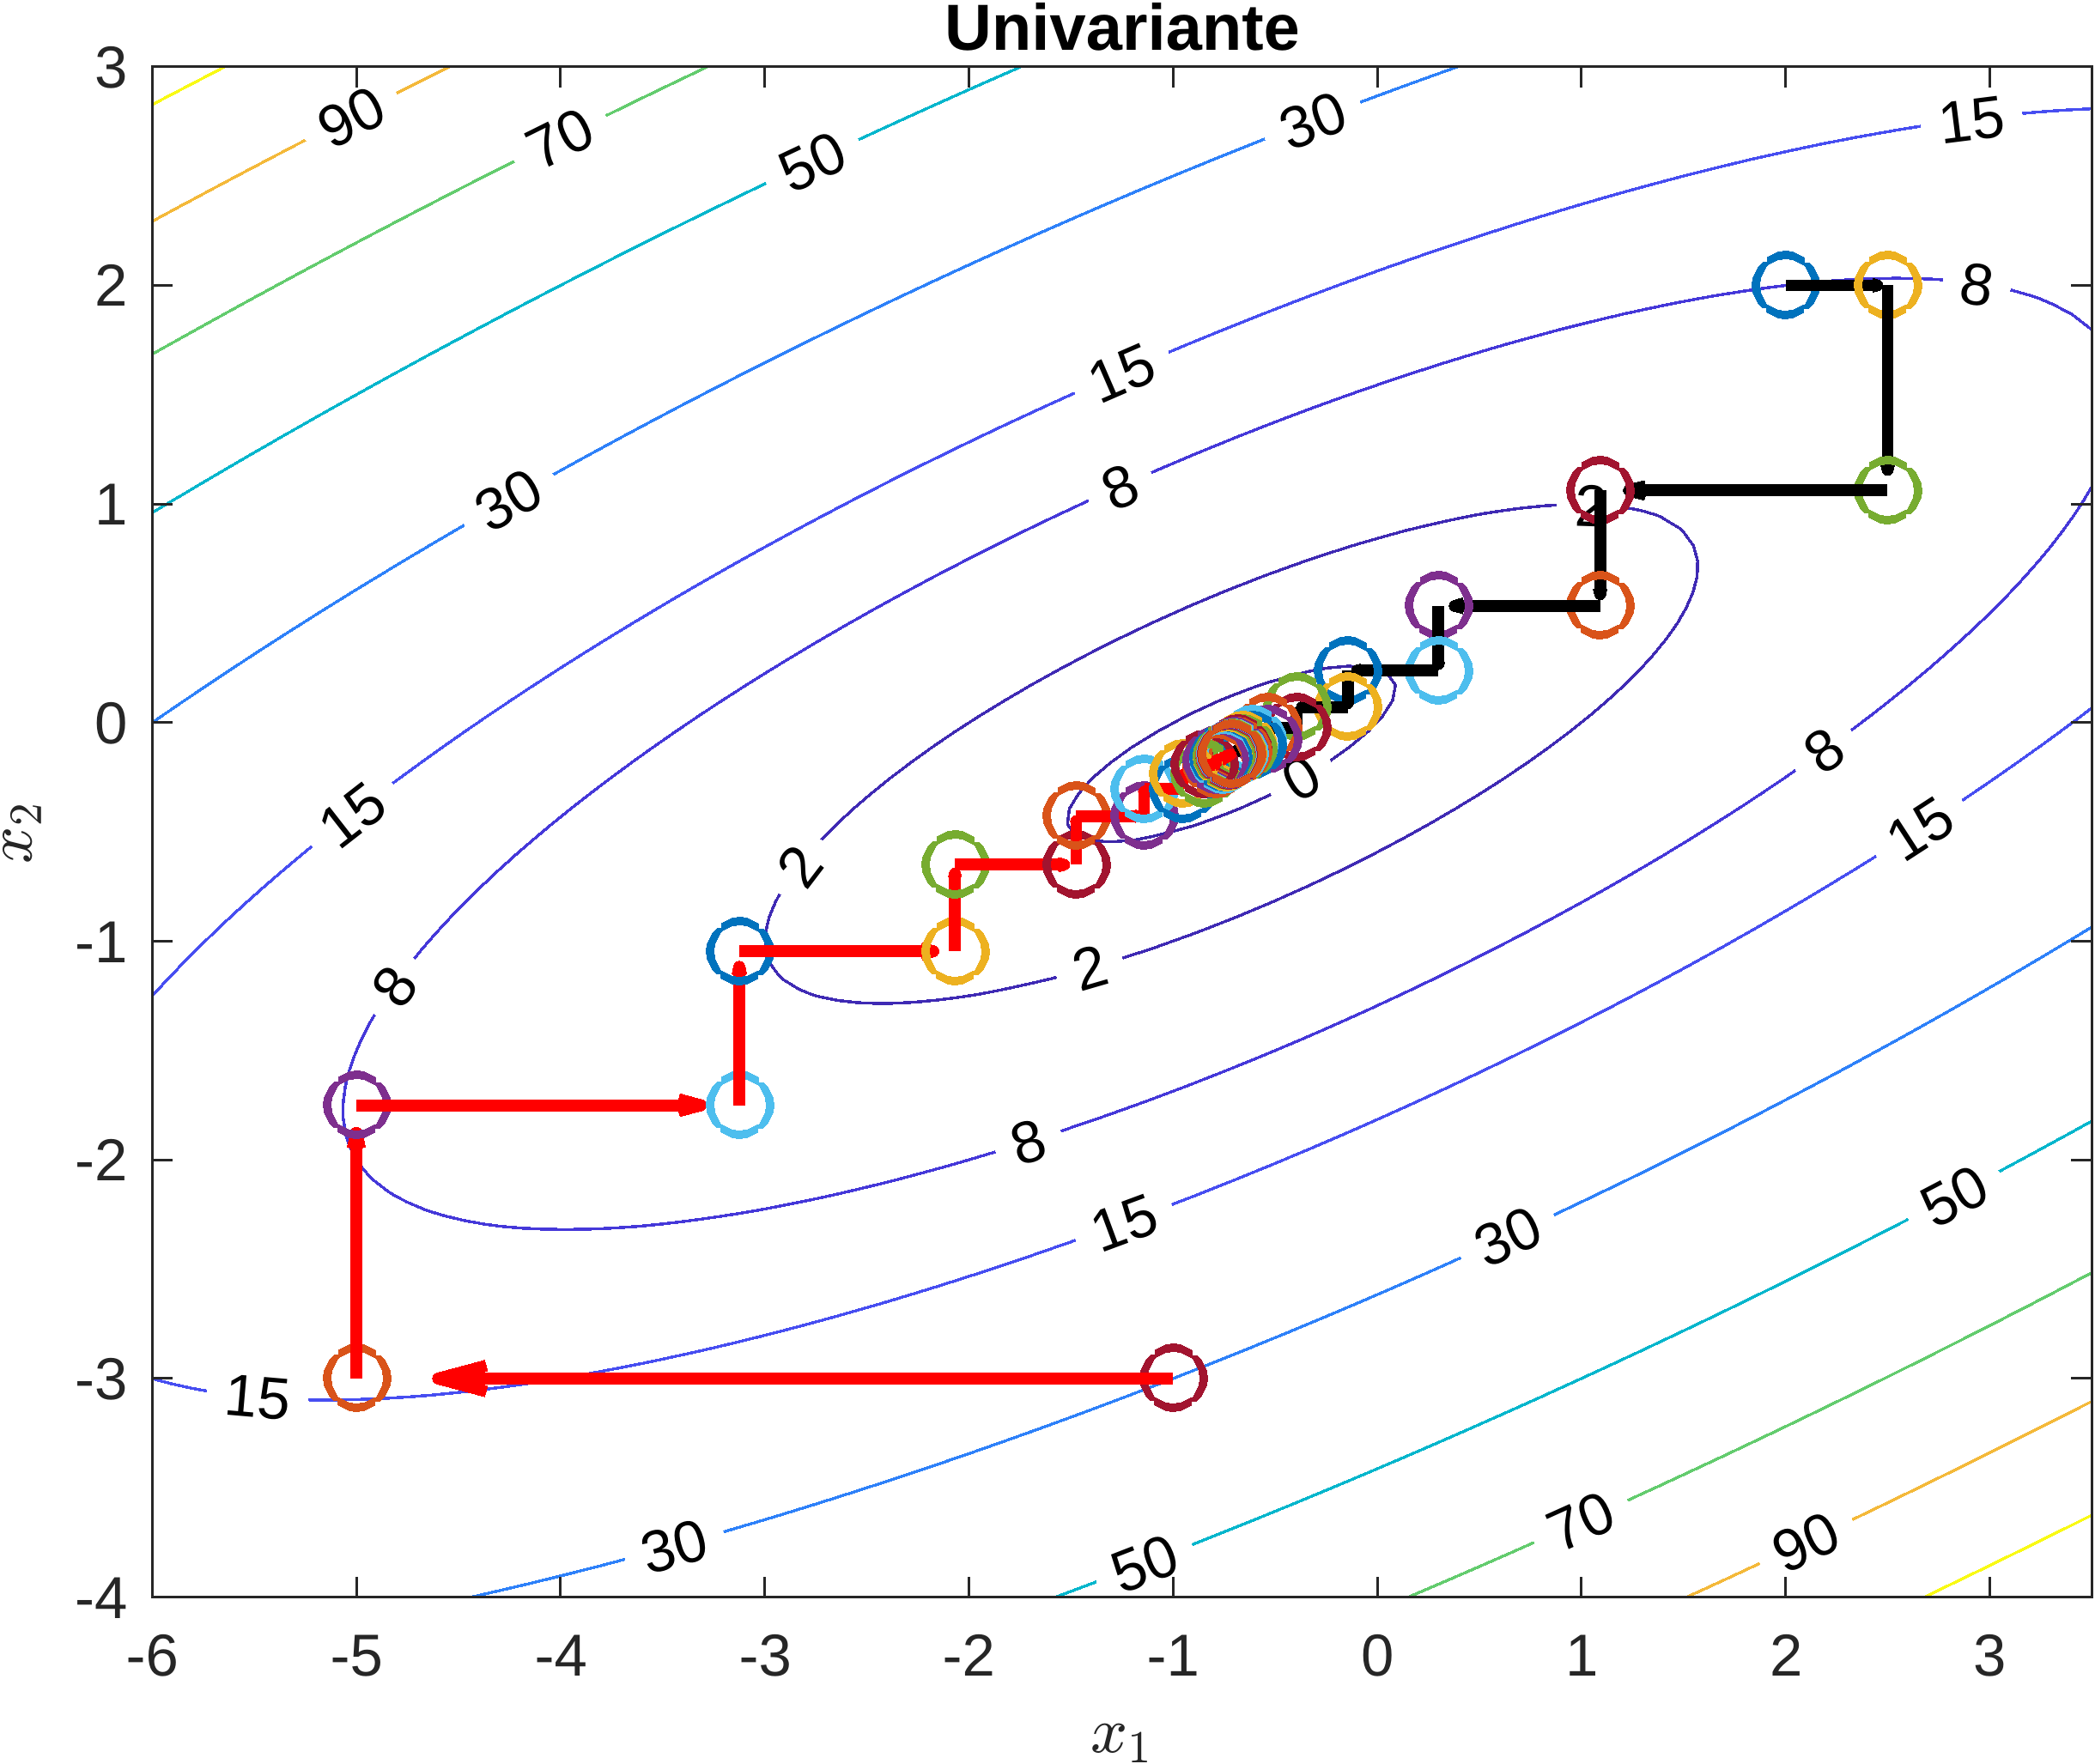
\includegraphics[width=\textwidth]{img01A_m01.png}
      \caption{Position (y) - real and estimated dsata}
      \label{fig:y}
\end{figure}

\begin{figure}[H]
      \centering
      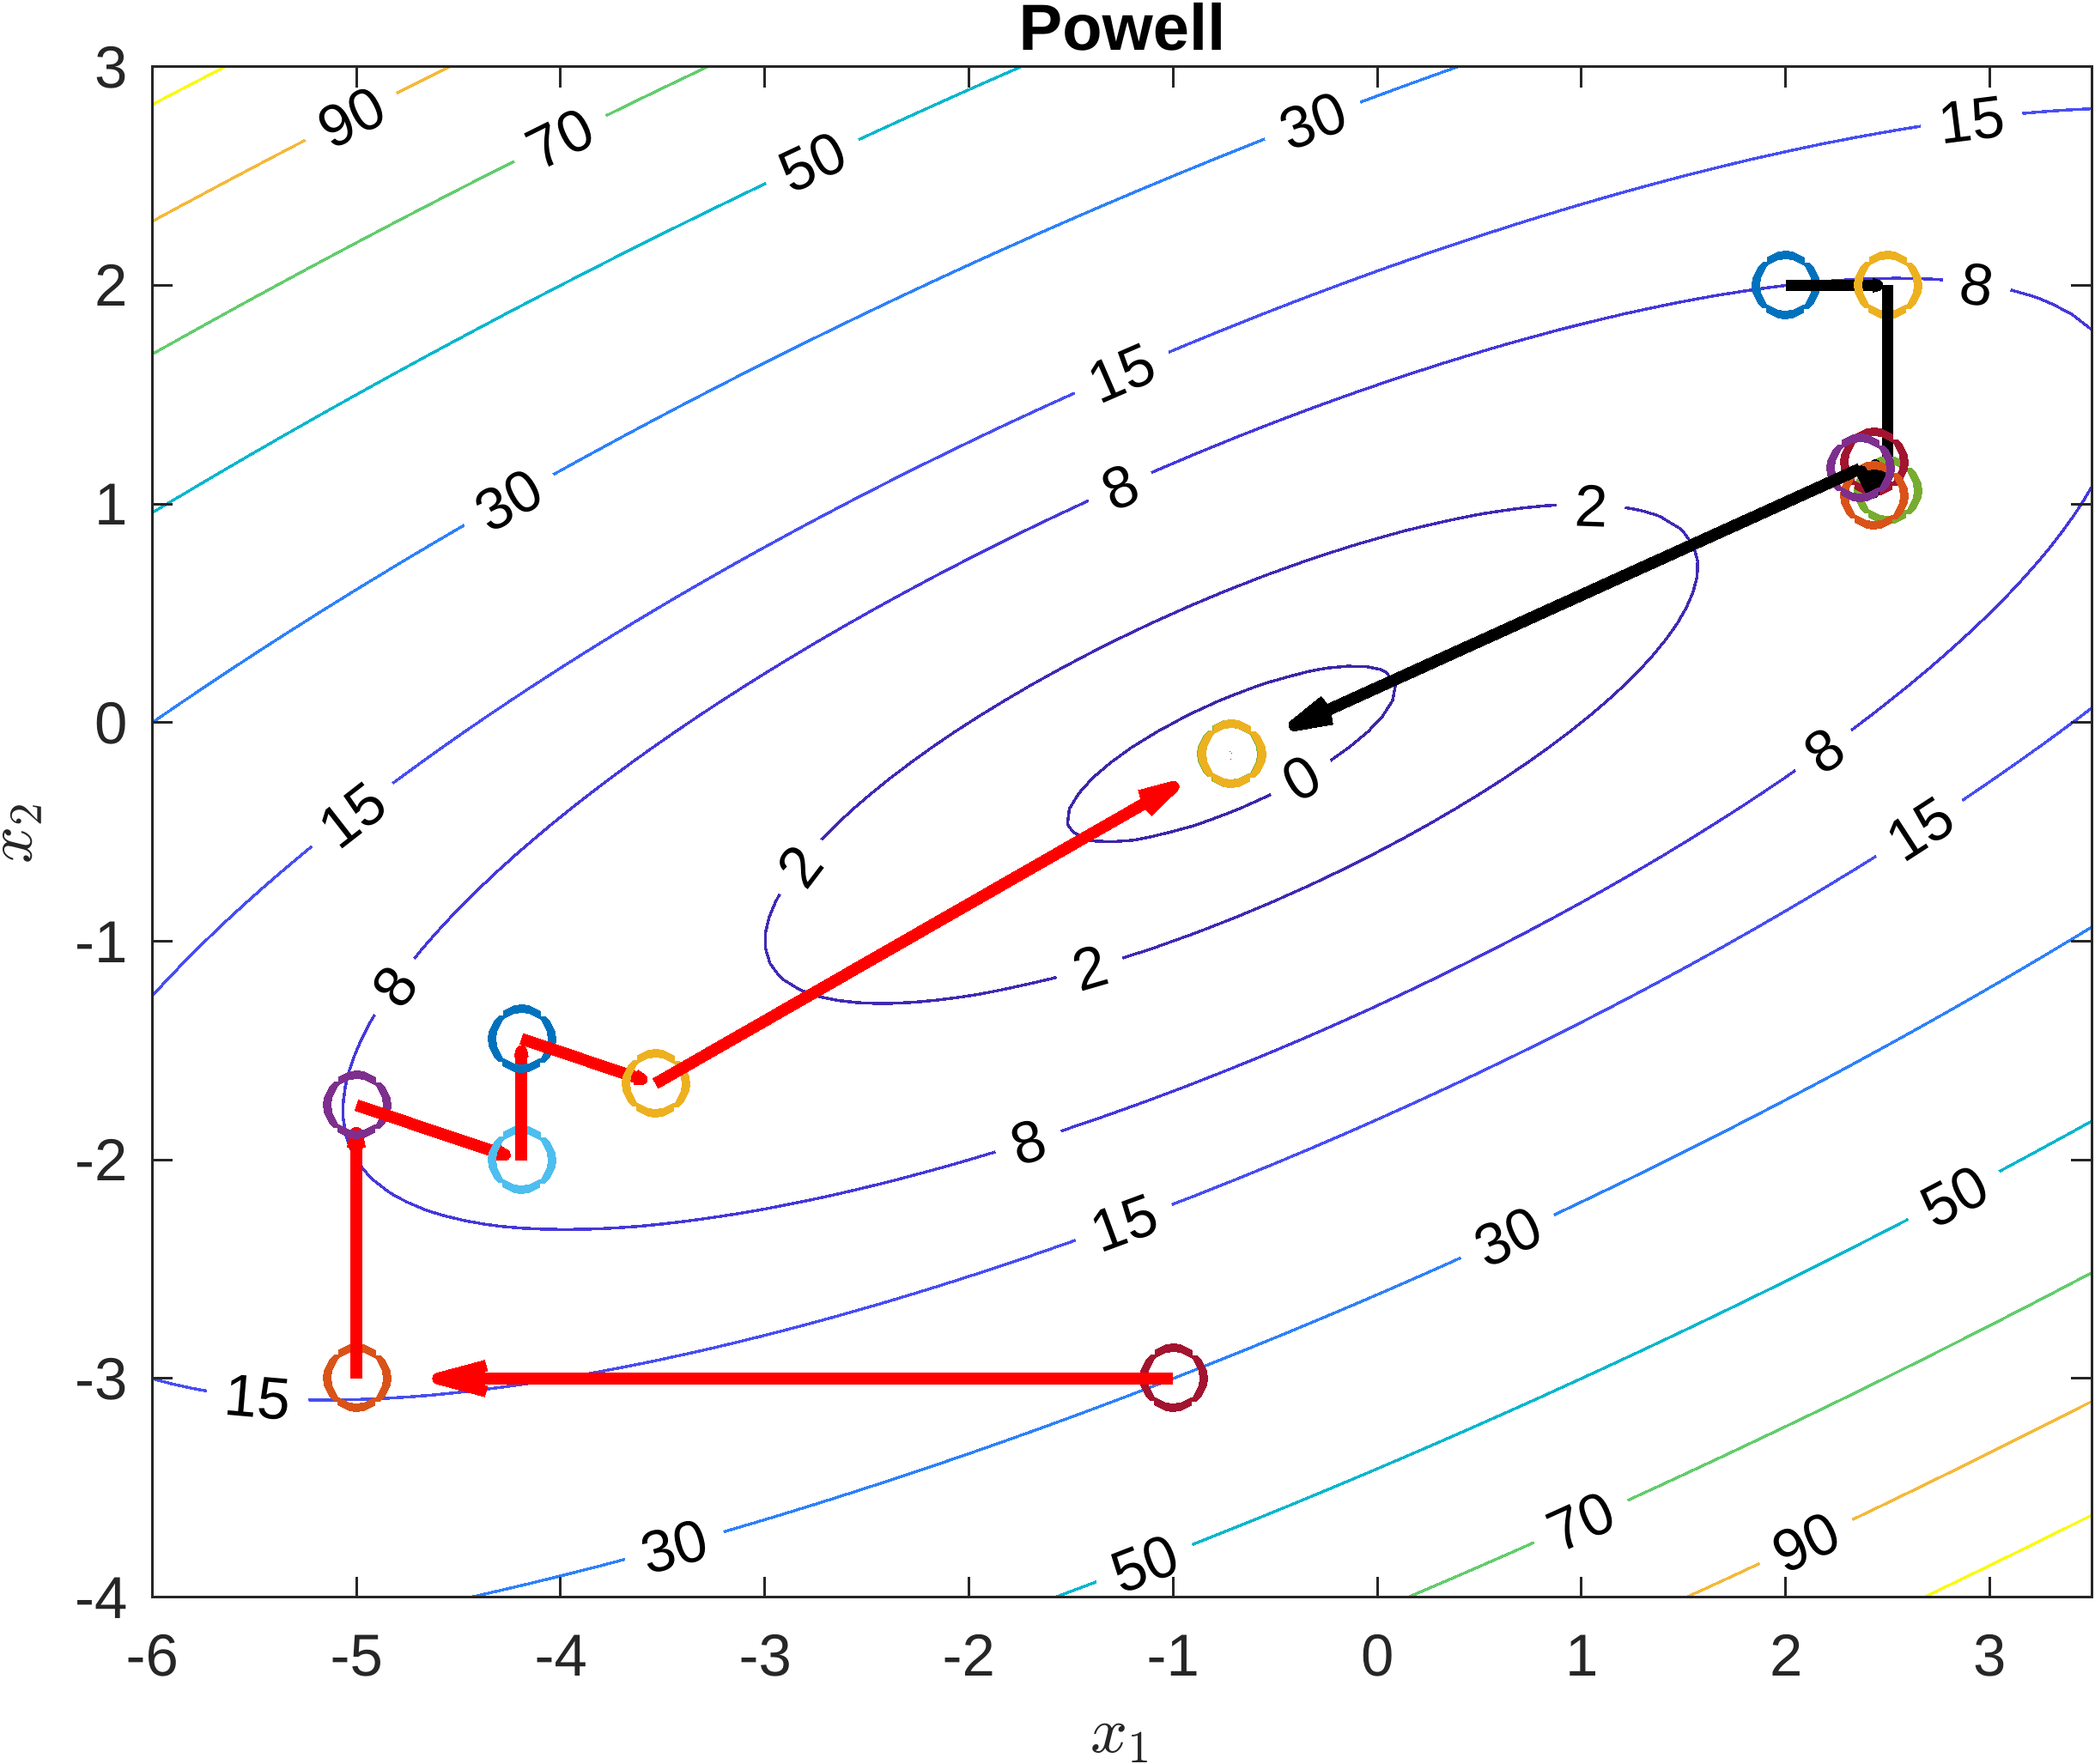
\includegraphics[width=\textwidth]{img01A_m02.png}
      \caption{Error between estimated and real data}
      \label{fig:e}
\end{figure}

\section{Anexos - C\'odigos}

asds


\begin{minipage}{\linewidth}
      \begin{lstlisting}[style=myStyle, caption=script t01.m setando par\^ametros e criando as fun\c c\~oes, label=l1]
            % dados do item 01a, f, grad f, hess f e x0
            fa = @(x) x(1)^2-3*x(1)*x(2)+4*x(2)^2+x(1)-x(2);
            gfa = @(x) [2*x(1)-3*x(2)+1 ; -3*x(1)+8*x(2)-1];
            Ha = @(x) [2 -3;-3 8];
            x01 = [2;2];
            x02 = [-1;-3];
            % parametros dos algoritmos
            iter_max = 100;
            a = 0.002; % passo
            TOL = 1e-4; % parada do gradiente
            TOL2 = 1e-7; % busca linear
            methods = ["Univariante","Powell","Steepest Descent","Fletcher Reeves","Newton-Raphson","BFGS"];
      \end{lstlisting}
\end{minipage}

\begin{minipage}{\linewidth}
      \begin{lstlisting}[style=myStyle, caption=script t01.m chamando o script osr.m para a fun\c c\~ao do item 1a para cada um dos 6 m\'etodos estudados, label=l2]
            fprintf('\n******************** ITEM 01A ************************\n');
            for method = 1:6
                fprintf('---%s---\n', methods(method));

                fprintf('x0=[%2d,%2d]: ',x01(1), x01(2));
                [x_1,t] = osr (fa, gfa, Ha, x01, method, iter_max, a, TOL, TOL2);
                fprintf('(%.1fms), xmin=[%0.4f,%0.4f], f=%0.4f\n', t*1000, x_1(1,end), x_1(2,end), fa(x_1(:,end)));

                fprintf('x0=[%2d,%2d]: ',x02(1), x02(2));
                [x_2,t] = osr (fa, gfa, Ha, x02, method, iter_max, a, TOL, TOL2);
                fprintf('(%.1fms), xmin=[%0.4f,%0.4f], f=%0.4f\n', t*1000, x_2(1,end), x_2(2,end), fa(x_2(:,end)));

                plot_result(min([x_1(1,:), x_2(1,:)])-dx,max([x_1(1,:), x_2(1,:)])+dx,min([x_1(2,:), x_2(2,:)])-dx,max([x_1(2,:), x_2(2,:)])+dx, x_1, x_2, methods(method), 1)
                exportgraphics(gcf,strcat('./figures/img01A_m0',num2str(method),'.png'),'Resolution',500)
            end
      \end{lstlisting}
\end{minipage}

\begin{minipage}{\linewidth}
      \begin{lstlisting}[style=myStyle, caption=script osr.m implementando o m\'etodo de Powell, label=list_osr]
            function [x_,time_elap] = osr (f, gf, H, x0, method, iter_max, a, TOL, TOL2)
            % 1. Univariante
            % 2. Powell
            % 3. Steepest Descent
            % 4. Flecher?Reeves
            % 5. Newton?Raphson
            % 6. BFGS

            k=0;
            conv=0; %flag convergencia
            tstart = tic;
            switch method
                case 2
                % 2. Powell
                    x_ = x0;
                    x = x0;
                    while k < iter_max
                        j = 1;
                        n = 2;
                        y = [[1;0],[0;1]];
                        while j <= n
                            [alpha_L, alpha_H] = passo_constante(f, x, y(:,1), a);
                            alpha_k = secao_aurea(f, x, y(:,1), TOL2, alpha_L, alpha_H);
                            k=k+1;
                            x = x + alpha_k*y(:,1);
                            x_ = [x_,x];
                            [alpha_L, alpha_H] = passo_constante(f, x, y(:,2), a);
                            alpha_k = secao_aurea(f, x, y(:,2), TOL2, alpha_L, alpha_H);
                            k=k+1;
                            x = x + alpha_k*y(:,2);
                            x_ = [x_,x];
                            d = x-x0;
                            [alpha_L, alpha_H] = passo_constante(f, x, d, a);
                            alpha_k = secao_aurea(f, x, d, TOL2, alpha_L, alpha_H);
                            k=k+1;
                            x0 = x + alpha_k*d;
                            x=x0;
                            x_ = [x_,x];

                            y(:,1) = y(:,2);
                            y(:,2) = d;

                            j = j+1;
                        end
                        if norm(gf(x)) < TOL
                            fprintf('%d steps!', k);
                            conv=1;
                            break;
                        end
                    end
                    if conv == 0
                        fprintf('Nao convergiu apos %d steps', k);
                    end
      \end{lstlisting}
\end{minipage}

\begin{minipage}{\linewidth}
      \begin{lstlisting}[style=myStyle, caption=script osr.m implementando o m\'etodo de Powell, label=list_passo_constante]
            function [alpha_L, alpha_H] = passo_constante(f, x0, d, a)
            alpha = 0;
            f_min = Inf;
            f_val = f(x0);
            alphas = [];
            f1 = f(x0 - a*d);
            f2 = f(x0 + a*d);
            if f1 < f2
                a=-a; % desce a esq (d-)
            end
            while f_val <= f_min
                x = x0 + alpha * d;
                f_val = f(x);
                if f_val < f_min
                    f_min = f_val;
                end
                alphas = [alphas; alpha];
                alpha = alpha + a;
            end
            alpha_L = alphas(end-1);
            alpha_H = alphas(end);
            if a < 0
                alpha_H = alphas(end-1);
                alpha_L = alphas(end);
            end
        end
      \end{lstlisting}
\end{minipage}

\begin{minipage}{\linewidth}
      \begin{lstlisting}[style=myStyle, caption=script osr.m implementando o m\'etodo de Powell, label=list_secao_aurea]
      function alpha_k = secao_aurea (f, x0, d, TOL, alpha_L, alpha_H)
            ra = (sqrt(5)-1)/2;
            b = norm(alpha_L-alpha_H);
            alpha_E = alpha_L + (1-ra)*b;
            alpha_D = alpha_L + ra*b;
            f1 = f(x0 + alpha_E * d);
            f2 = f(x0 + alpha_D * d);
            while b > TOL
                  if f1 > f2
                        alpha_L = alpha_E;
                        alpha_E = alpha_D;
                        b = norm(alpha_L-alpha_H);
                        alpha_D = alpha_L + ra*b;
                        % avaliar menos vezes a funcao f
                        f1 = f2;
                        f2 = f(x0 + alpha_D * d);
                  else
                        alpha_H = alpha_D;
                        alpha_D = alpha_E;
                        b = norm(alpha_L-alpha_H);
                        alpha_E = alpha_L + (1-ra)*b;
                        % avaliar menos vezes a funcao f
                        f2 = f1;
                        f1 = f(x0 + alpha_E * d);
                  end
            end
            alpha_k = (alpha_L+alpha_H)/2;
      end
      \end{lstlisting}
\end{minipage}

\end{document}
